\chapter{State of the Art}
\label{chap:state_of_the_art}
\setcounter{section}{0}
\setlength{\parskip}{0.6em}
\section{Symbolic Artificial Intelligence}
\label{sec:symbolic_ai}


Symbolic Artificial Intelligence represents the foundational paradigm that laid the foundations for the field during the mid-20th century until the late 1980s. This deterministic approach is based on \textit{Physical Symbol System Hypothesis}, formulated by Allen Newell and Herbert Simon in 1976 \cite{NewellSimon1976}. This approach aims to represent human knowledge through symbols and states, it represents real world concepts where you can manipulate these using logical rules to solve problems.


Unlike sub-symbolic AI that learns from vast datasets to better understand real world data, symbolic systems are designed from the ground up to tackle only certain domains. Developers have to manually encode rules and constraints related to such domain into a format that the machine understands. This makes the \textit{reasoning process} transparent and interpretable, knowing which actions it took and why, meaning that every decision can be tracked to its origin state, unlike current sub-symbolic AI models where there is an almost unexplainable black box.


Historically, symbolic AI has come has made tremendous breakthroughs such as the \textit{Logic Theorist} (1956), these systems demonstrated that machines could perform expert-level tasks in narrow domains by following a sequence of logical rules. However, they stills faced some key challenges, as seen in the \textit{AI Winter}, handling uncertainty and learning from experience. However the automated planning and the knowledge representation are still at an advantage with the deterministic and long-term planning it offers, against sub-symbolic AI.


In the context of this project, symbolic AI can give a huge advantage over reasoning the series of steps to follow to perform a certain GUI-Actions, from opening an app to sending an email. Making this a deterministic approach, by using PDDL (Planning Domain Definition Language). Therefore the system can generate structured and traceable sequences of actions to navigate graphical interfaces, ensuring that the agent’s behaviour is logical, with a specific goal and deterministic, features which sub-symbolic AI may lack.


{
\interlinepenalty=10000
To achieve this desired behaviour, Symbolic AI relies heavily on Knowledge representation. The most common methodology involves First-Order Logic, which uses predicates and quantifiers to describe the world around us and the relationship between objects, for instance the relationship between a parent and a child folder in order to correctly navigate through them. This architecture was popularized by \textit{Expert Systems}, this established a clear separation between the \textit{Knowledge Base} and the \textit{Inference Engine}, which makes the entire codebase scalable, so there is no need to rewrite the logic every time the knowledge is updated.
\par
}


Within this logical framework, Automated Planning emerged as the specific sub-field dedicated to generating action sequences. The foundation of modern planning is the STRIPS (Stanford Research Institute Problem Solver) system from the early 1970s \cite{FikesNilsson1971}, which introduced the concept of defining actions via preconditions and effects. This means declaring certain conditions that must be true to execute an action, and how the state changes afterward. Mathematically, an action $a$ defines a state transition function $\gamma(s, a)$. If the preconditions are met in the current state $s$ ($Pre(a) \subseteq s$), the new state is computed as:


\begin{equation}
    \gamma(s, a) = (s \setminus Del(a)) \cup Add(a)
\end{equation}


\noindent This implies that the next state is derived by removing the "delete effects" ($Del(a)$) from the current state and adding the "add effects" ($Add(a)$). This logic evolved into the Planning Domain Definition Language (PDDL), which is now the standard research tool for AI planning \cite{McDermott1998}. PDDL allows for a rigorous definition of the domain and problem. Formally, a classical planning task can be defined as the 4-tuple:


\begin{equation}
    \Pi = \langle \mathcal{F}, \mathcal{A}, \mathcal{I}, \mathcal{G} \rangle
\end{equation}


\noindent Where:
\begin{itemize}
    \item $\mathcal{F}$ is a finite set of facts describing the state of the world (e.g. \textit{window\_open}).
    \item $\mathcal{A}$ is a finite set of deterministic actions the agent can perform (e.g. \textit{type\_text}).
    \item $\mathcal{I} \subseteq \mathcal{F}$ represents the Initial State, defining what is true at the start.
    \item $\mathcal{G} \subseteq \mathcal{F}$ represents the Goal State, defining the conditions that must be true to finish.
\end{itemize}

A domain is where you declare the set of actions $\mathcal{A}$, such as clicking, typing, opening an app… Whereas the definition of a problem is where you initialise a set of states and objects and a desired goal. By standardizing these definitions, PDDL enables the creation of agents that can reason about GUI interactions as logical transitions rather than probabilistic guesses. This transition process, where preconditions determine the applicability of actions to transform the system state, is visualized in Figure \ref{fig:pddl_workflow}.
\begin{figure}[H]
    \centering
    % Ajusta el ancho al 80% del texto (puedes cambiar 0.8 por 0.5, 1.0, etc.)
    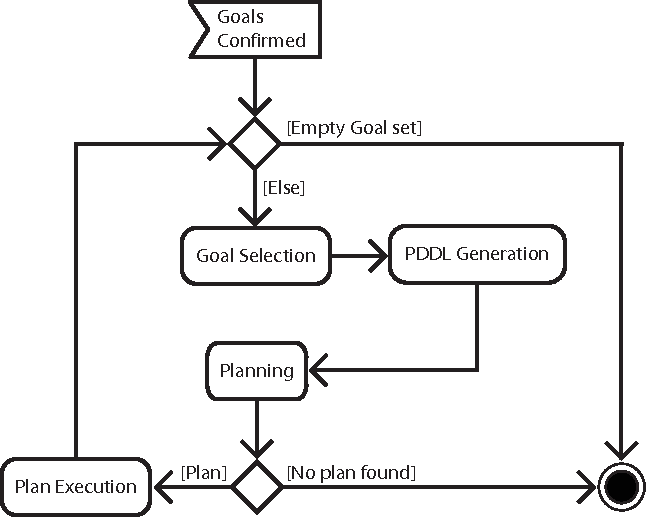
\includegraphics[width=0.5\textwidth]{images/pddl_diagram.png}
    \caption{Workflow of the Planning System.}
    \label{fig:pddl_workflow}
\end{figure}

The PDDL workflow has to start a with goal confirmation, followed by plan generation using search algorithms, such as Breadth First Search, Greedy Best First Search and A*. If a valid plan is found, it proceeds to execution, otherwise, the cycle may restart and choose another path to follow or end without any path found.

However, defining the domain and problem is only the first step, the key challenge is to find the optimal sequence of actions, which requires efficient search algorithms. Classical planning treats the task as a search through a state space, exploring paths from the initial state to the goal. In complex domains like in a GUI interaction system, the state space grows exponentially, this leads to combination of states where an exhaustive search becomes unfeasible. To address this, three main categories of search algorithms are typically considered:


\begin{enumerate}
    \item \textbf{Breadth-First Search (BFS):} This algorithm explores the closer neighbor nodes first, before moving to the next level neighbors. While it guarantees finding the shortest path (optimality), it is computationally expensive as it expands every possible state blindly ($f(n) = g(n)$), making it impractical for large state spaces (complex user tasks).
    
    \item \textbf{Greedy Best-First Search:} This approach prioritizes nodes that appear to be closest to the goal ($f(n) = h(n)$). It is generally faster than BFS it is not optimal. It can find a plan, but it isn’t the most optimal or efficient making it redundant.
    
    \item \textbf{A* (A-Star) Search:} It combines the strengths of the previous two approaches by minimizing a total cost function that balances the actual path cost incurred so far with an intelligent estimate of the remaining cost to the goal \cite{Hart1968}:
    \begin{equation}
        f(n) = g(n) + h(n)
    \end{equation}
    \noindent Where $g(n)$ is the actual cost from the start node to node $n$, and $h(n)$ is the heuristic estimated cost from $n$ to the goal.
\end{enumerate}


To ensure both efficiency and optimality (unnecessary opened apps or clicks), this project relies on A* search. Specifically, it utilizes Fast Downward \cite{Helmert2006}, a state-of-the-art planning system developed by Malte Helmert that has consistently achieved top performance in International Planning Competitions.


Fast Downward is particularly well-suited for this project because of its robust implementation of the LM-cut heuristic (Landmark Cut). This advanced technique analyzes the problem structure to identify \textit{landmarks}, which are facts that must become true at some point in any valid plan to reach the goal. For example, to open a file inside the Documents folder, the system must first navigate to Documents, this navigation is a compulsory landmark.


By calculating the minimum cost of achieving these obligatory intermediate states, LM-cut provides a heuristic that never overestimates the remaining cost. This mathematical property guarantees that Fast Downward finds the optimal plan for the sequence of GUI actions. This optimality is critical as it reduces the number of unnecessary clicks, types and open applications, reducing the surface error area.


Despite these strengths in logical reasoning and planning, Symbolic AI suffers from a critical limitation known as the \textit{Symbol Grounding Problem}. While the planner knows the sequence of actions to execute a task, such as "click the Chrome icon," it has no inherent way to perceive where that icon is located on the screen. It operates on abstract labels, blind to the computer interface. This gap creates a need for Sub-Symbolic AI, which can process unstructured data and bridge this gap between the real world and the logical domain system in PDDL.


\clearpage
\section{Sub-Symbolic Artificial Intelligence}
\label{sec:sub-symbolic_ai}



Sub-Symbolic Artificial Intelligence systems are the next step on machines interacting with the real world. While symbolic AI relies on an explicit declaration of the domain with certain logic rules, objects and goals, Sub-Symbolic AI learn from past experiences (training data) which are representations of the specific domain, so later in a real world test they can behave according to what they saw before. This mimics the human brain, where the model learns from the bottom‑up, extracting patterns from raw data \cite{Rosenblatt1958}.



This is the predominant approach made with Neural Networks, which are computational nodes (neurons) composed of specific layers. This creates a clear distinction between the previous deterministic behaviour mentioned with heuristic algorithms and the creation of relationships which are probabilistic and continuous. Information is not stored in the \textit{Knowledge Base}, but is distributed across the network’s weights that determine the strength of the connection. Therefore, it can generalize from a constructed dataset, understanding ambiguity, noise and incomplete data, where symbolic AI fails to achieve \cite{Rumelhart2002}.



Mathematically, the fundamental unit of these networks, the artificial neuron, processes an input vector $\mathbf{x}$ through a weighted sum and a non-linear activation function $\phi$. This formalizes how the weights modify the output based on the input, allowing the network to learn complex patterns:



\begin{equation}
    \hat{y} = f \left( \sum_{i=1}^{n} (w_n \cdot x_n) + b \right)
\end{equation}


\noindent Where:
\begin{itemize}
    \item $\hat{y}$ is the output (predicted value).
    \item $f()$ is the activation function.
    \item $w_n$ represents the weights.
    \item $x_n$ represents the input features.
    \item $b$ is the bias term.
\end{itemize}



\begin{figure}[H]
    \centering
    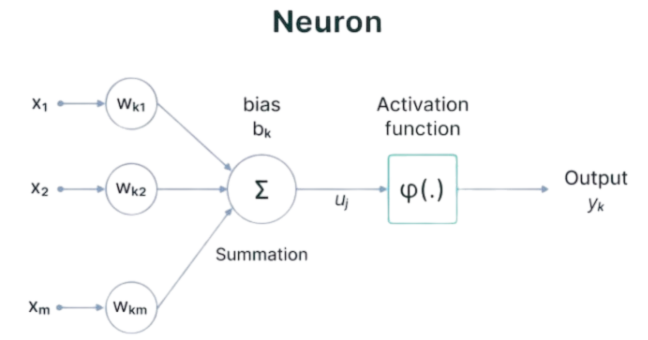
\includegraphics[width=0.5\textwidth]{images/perceptron.png} 
    \caption{An Artificial Neuron where inputs ($x$) are weighted ($w$), summed, and activated to produce an output ($y$).}
    \label{fig:neuron_model}
\end{figure}



However, a single neuron is limited in its capacity to solve complex problems, for instance, it cannot solve non-linear problems like XOR without layers. To address this, neurons are arranged in layers to form a \textit{Multi-Layer Perceptron} (MLP) or Deep Neural Network.



\begin{figure}[H]
    \centering
    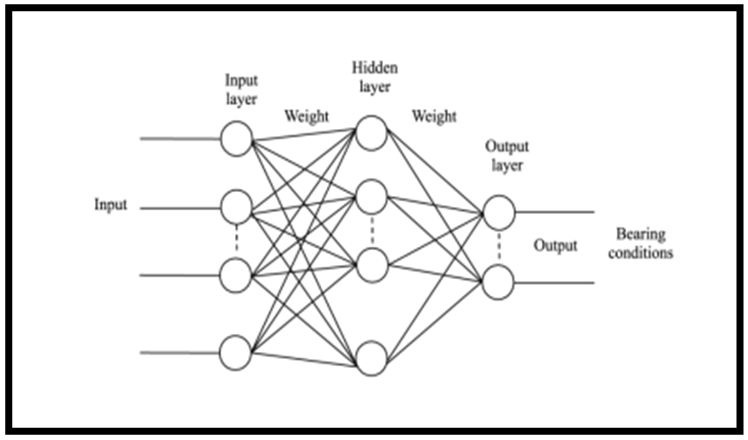
\includegraphics[width=0.5\textwidth]{images/neural_network.jpg} 
    \caption{Architecture of a Deep Neural Network. The system consists of an Input Layer, multiple Hidden Layers for feature extraction, and an Output Layer for final prediction.}
    \label{fig:deep_network}
\end{figure}



This layered architecture is the foundation of the modern models used in this project. Specifically, it enables the use of Large Language Models (LLMs) or Small Language Models (SLMs) for reasoning and Vision-Language Models (VLMs) for perception. These advanced sub-symbolic systems serve as the interface between the user's intent and the symbolic planner, effectively solving the Symbol Grounding Problem described in the previous section. Recent work has explained that symbolic and sub-symbolic methods are not exclusive but can be combined into hybrid architectures that exploit the strengths of both \cite{IlkouKoutraki2020}.
